\section{压力测试}
从github上获取redis 2.4的版本仓库用于测试git与sit的时空效率。
\subsection{测试方法}
在redis中以master分支为基准,找出一条版本链,如果这个版本是merge得到的,那么就选择它的第一个父版本。然后将版本链上的每一个版本checkout,然后执行add和commit命令,同时监控其CPU时间的消耗。
\subsection{空间占用}
把所有的文件都add和commit到仓库中后分别查看``.sit''和``.git''文件夹的大小。
\begin{center}
\begin{tabular}{|l|r|r|}
\hline
                         & 仓库大小 & 相对大小\\
\hline
.git                     & 94324 kB           &   100\% \\
\hline
.sit(with compression)   & 82180 kB           &  87.1\% \\
\hline
.sit(without compression)& 264004 kB          & 279.9\% \\
\hline
\end{tabular}
\end{center}
\subsection{时间使用}
比较了sit(有无压缩功能)与git的时间效率(结果见后图)。
\begin{figure}[H]
	\centering
	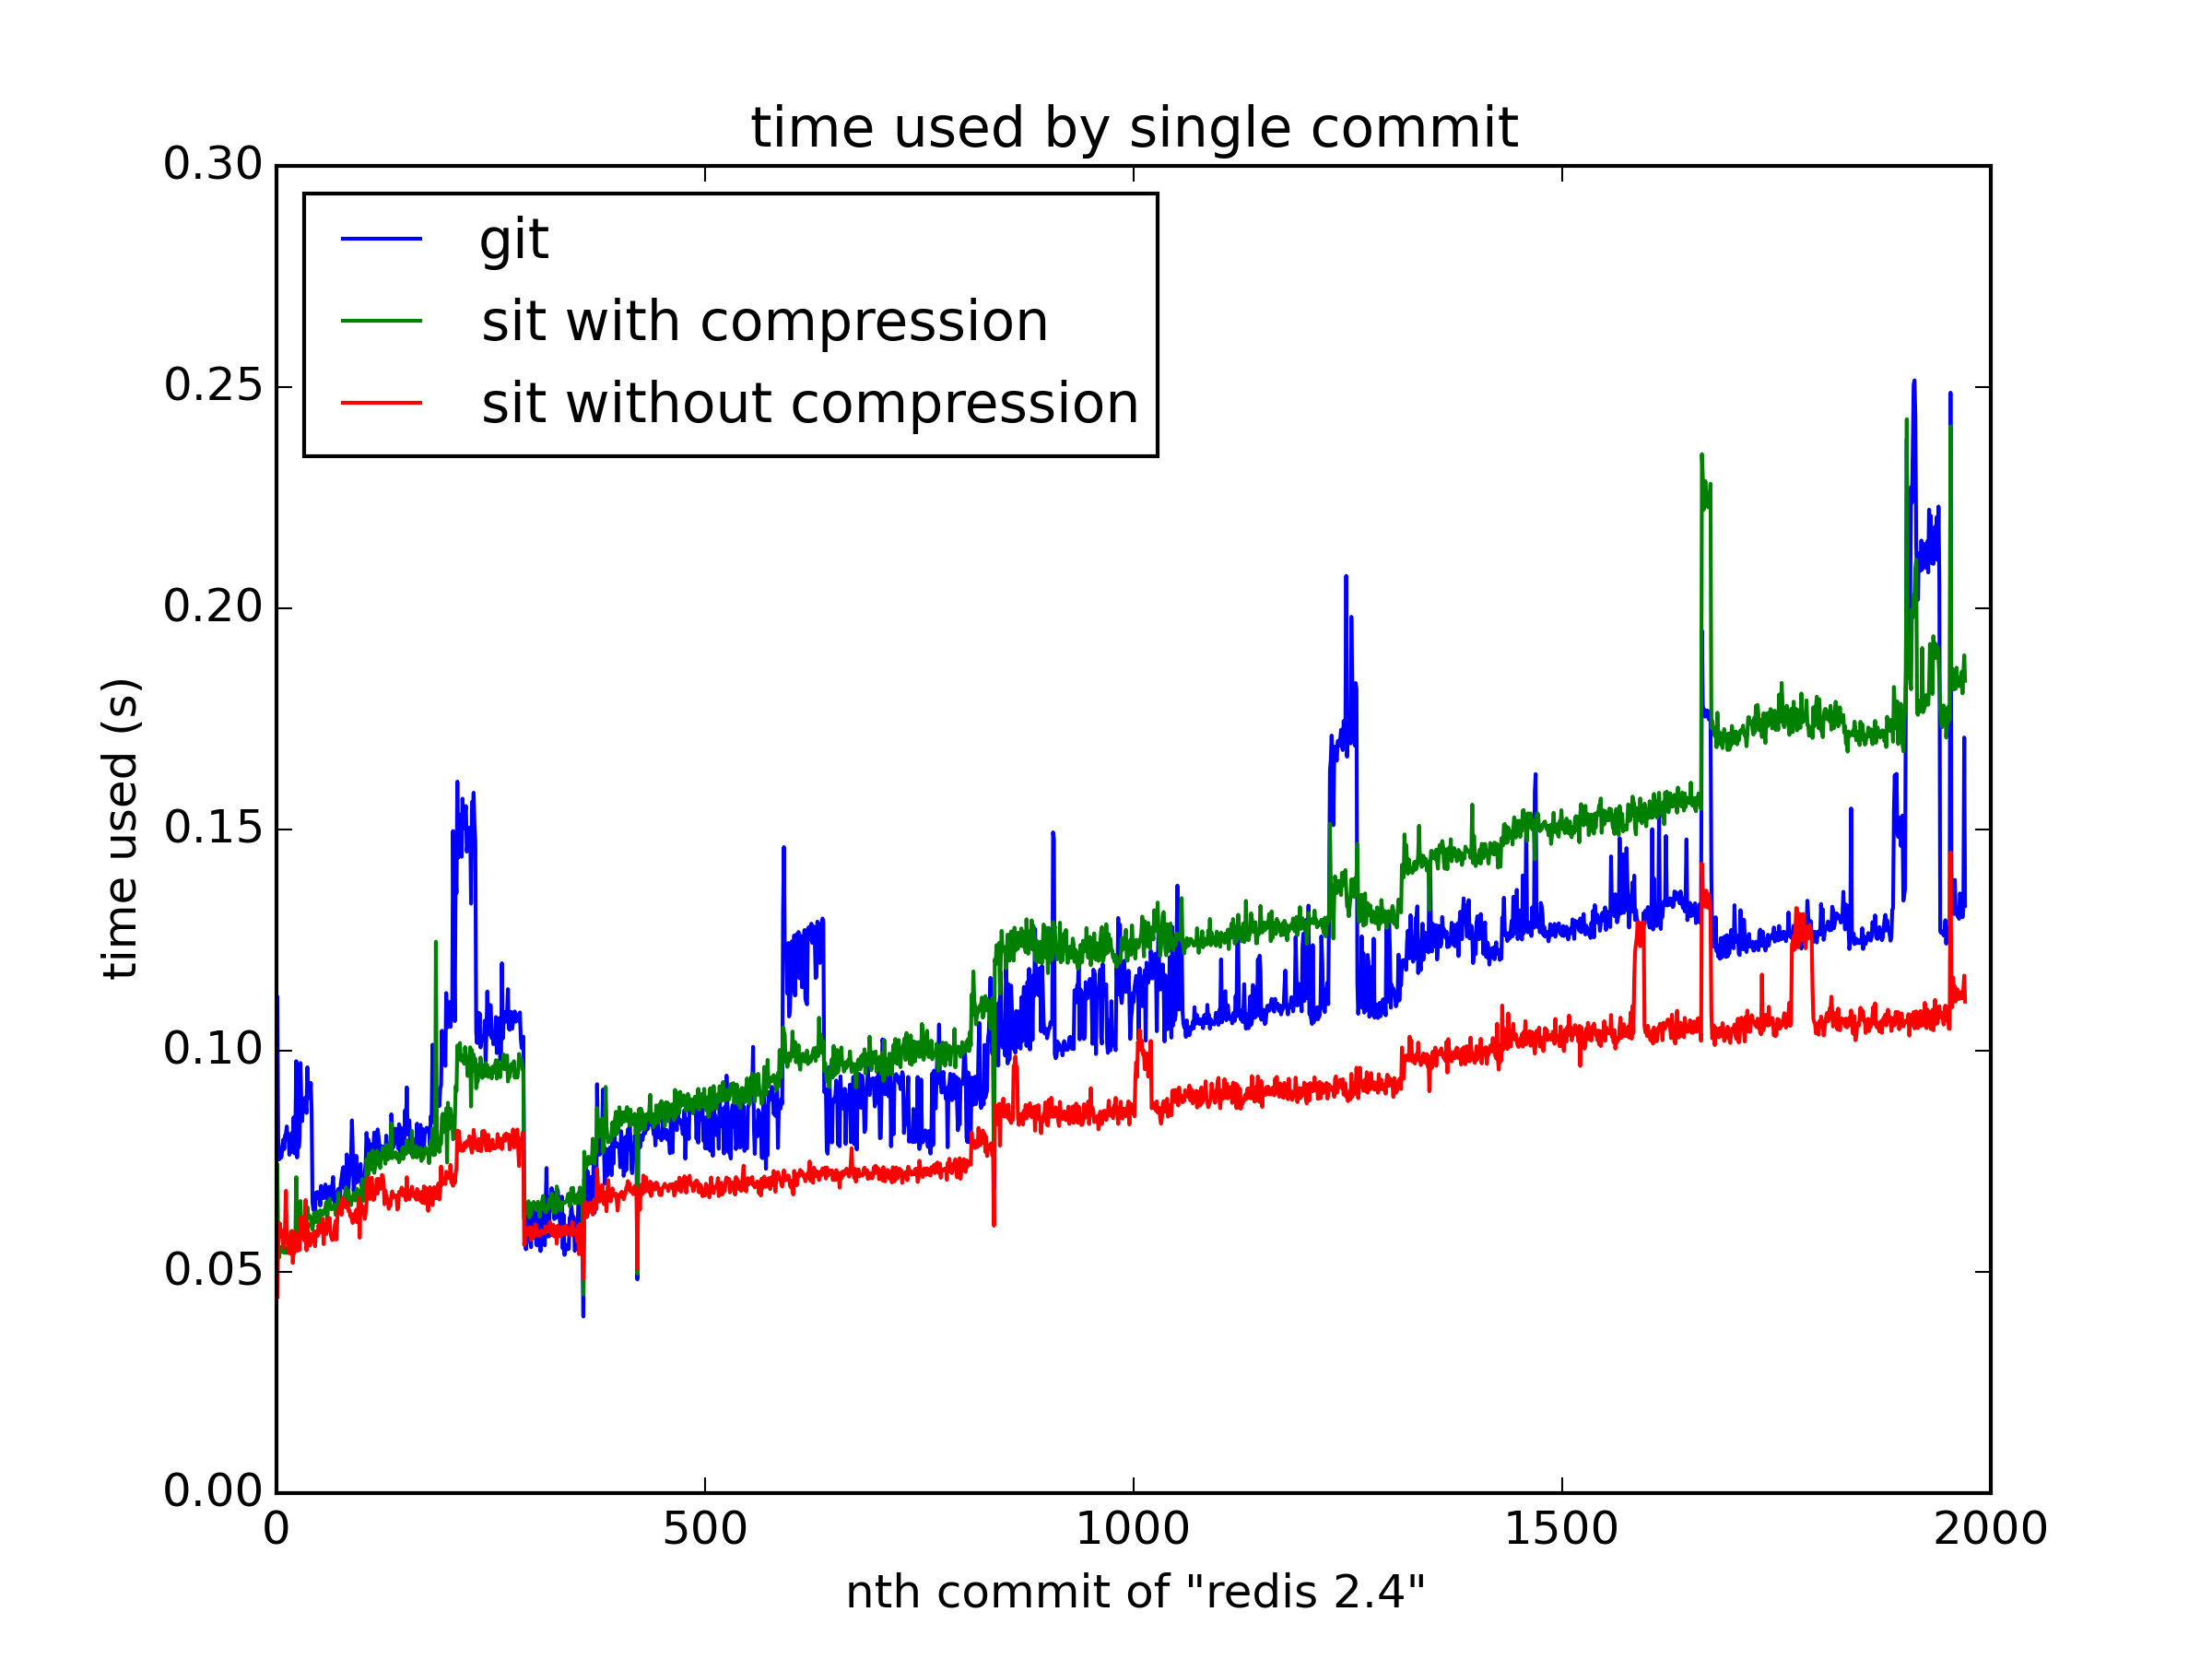
\includegraphics[scale=0.7]{figure_1.png}
	\caption{单次commit操作所需要的时间}
\end{figure}
\begin{figure}[H]
	\centering
	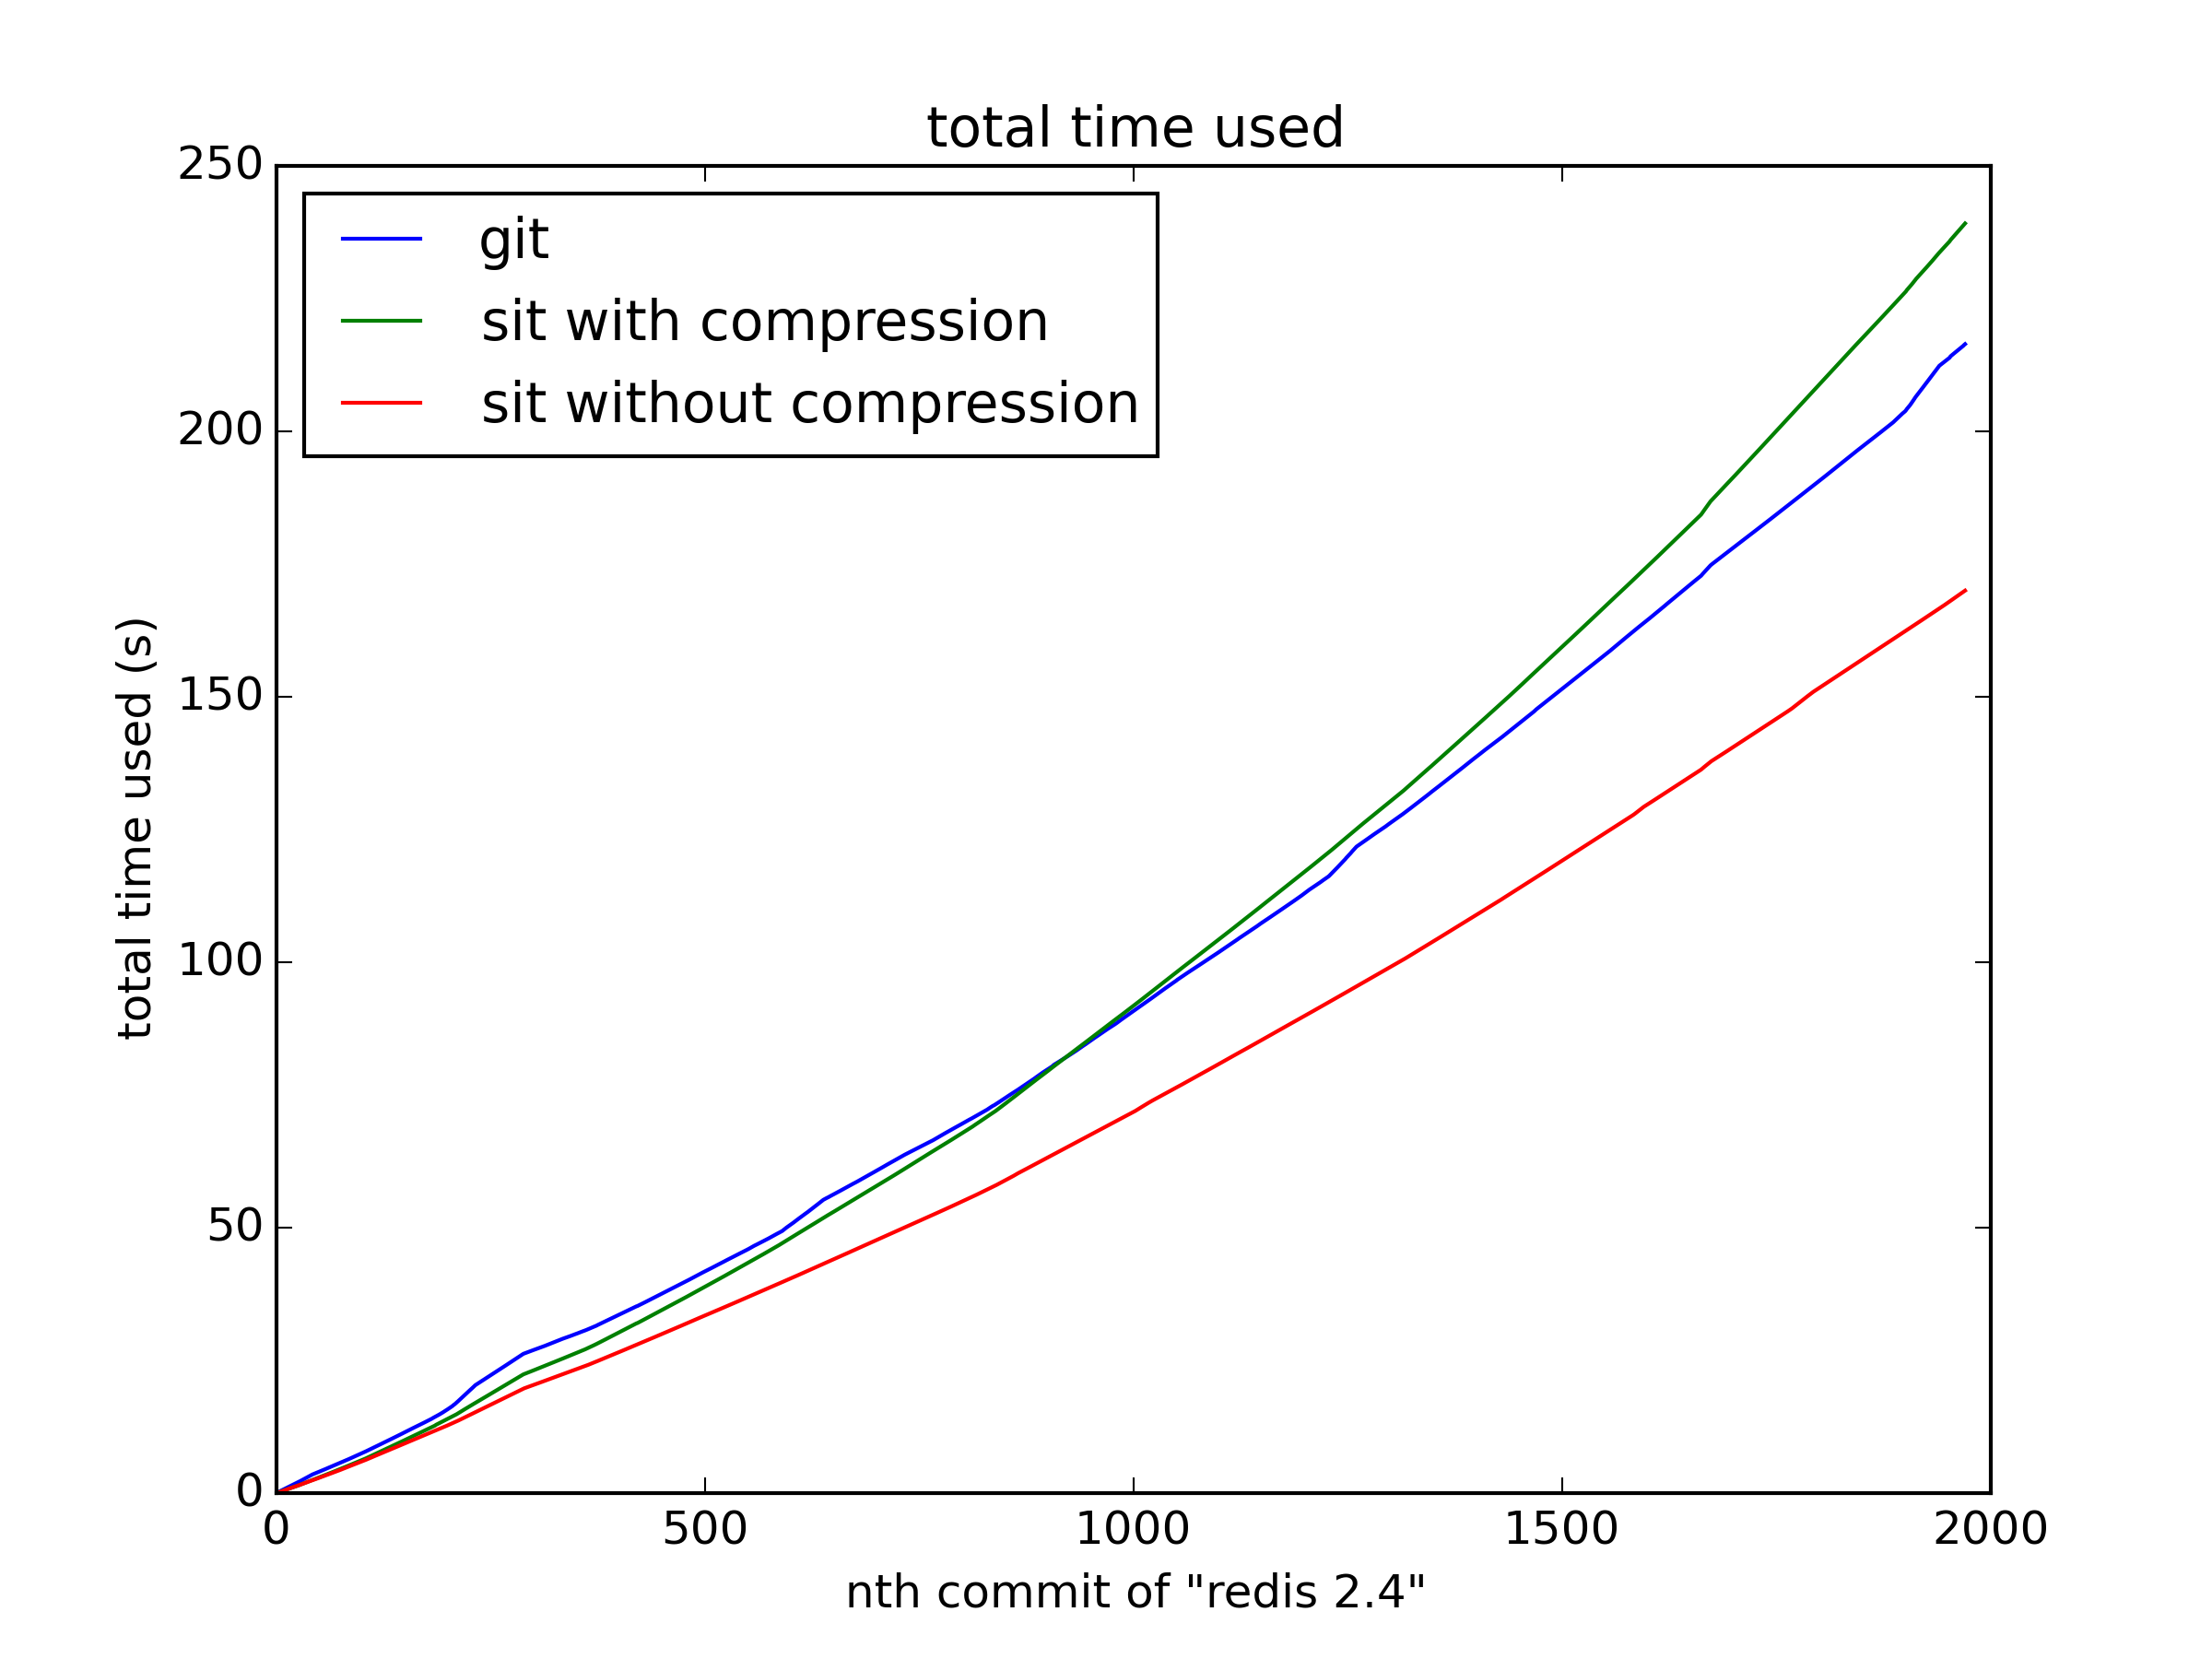
\includegraphics[scale=0.7]{figure_2.png}
	\caption{耗去的总时间}
\end{figure}
\subsection{结论}
从时间和空间的测试结果可以初步得出结论:在不支持压缩时,sit快于git,但仓库占用的空间约为git的2.8倍;支持压缩的sit的运行速度明显下降,低于git,但是在空间效率上升,优git更好。